\documentclass{article} 
\usepackage{amsmath,amssymb, stmaryrd}
\usepackage{tikz}
\usepackage{comment}
\usepackage{amsthm}
\usetikzlibrary{arrows,decorations.pathmorphing,backgrounds,fit}
\usetikzlibrary{shapes.geometric}
\usepgflibrary{shapes.geometric}
\usetikzlibrary{shapes.symbols}
\usepgflibrary{shapes.callouts}
\usetikzlibrary{shapes.callouts}

\newcommand{\BD}[1]{\mathrm{BD}(#1)}
\newcommand{\DMA}[2]{\mathrm{DMA}(#1,#2)}

\title{Hybrid Automata}
\date{\today}


%%% Authors are given together with their institut.

\author{ 
   Andrew Lawrence}

\begin{document}
\maketitle


\begin{center}
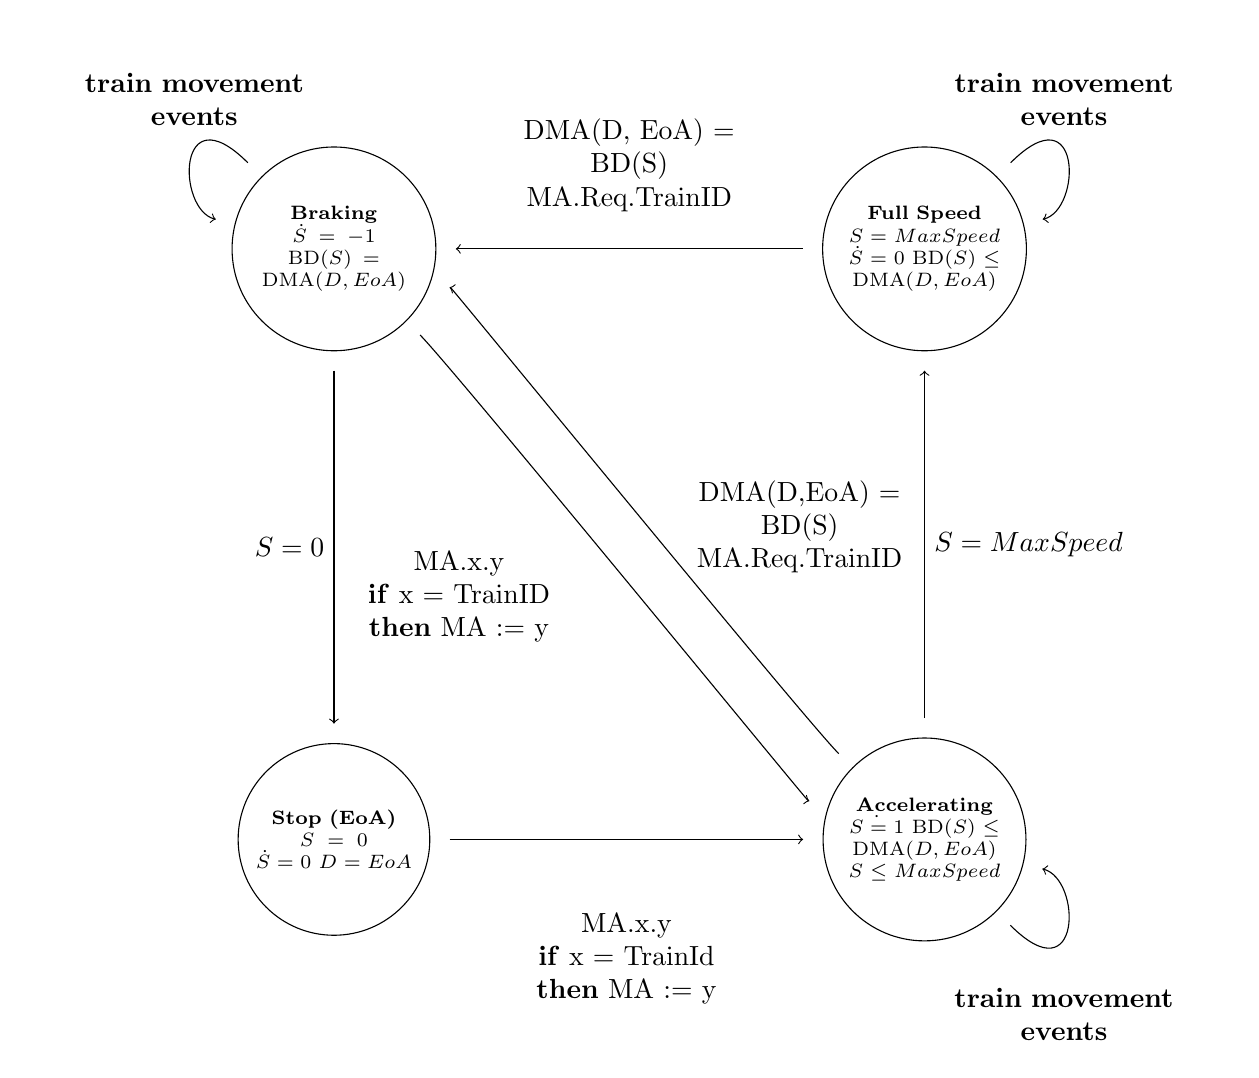
\begin{tikzpicture}[node distance = 2cm]

\tikzstyle{box1}=[circle, draw, text width = 2cm, font=\scriptsize, text centered]
\tikzstyle{arrow}=[->,shorten >=7pt,shorten <= 7pt]
\tikzstyle{biarrow}=[<->,very thick,shorten >=7pt,shorten <=7pt]


\node (A) [box1]  at (0,0)                  {\textbf{Stop (EoA)} \\
							$S = 0$ \\
                                                        $\dot{S} = 0$
							$D = EoA$ 

                                            };

\node (B) [box1]    at (7.5,0)          { \textbf{Accelerating} \\
       $\dot{S = 1}$
       $\BD{S} \leq \DMA{D}{EoA}$
       $S \leq MaxSpeed$
};

\node (C)[box1] at (0, 7.5)  { \textbf{Braking}\\
					                   $\dot{S} = -1$ 
						           $\BD{S} = \DMA{D}{EoA}$
                                               
						};

\node (D)[box1] at (7.5, 7.5)  { \textbf{Full Speed }\\
					                   $S = MaxSpeed$
                                                            $\dot{S} = 0$
							    $\BD{S} \leq \DMA{D}{EoA}$             
						};


\draw [arrow] (B) -- node[right] {$S = MaxSpeed$} (D);
\draw [arrow] (A) -- node[below = 10pt, text width = 4cm] {\begin{center}MA.x.y\\ \textbf{if} x = TrainId\\ \textbf{then} MA := y\end{center} } (B);
\draw [arrow] (D) --  node[above = 10pt,text width=4cm] {\begin{center}DMA(D, EoA) =\\ BD(S)\\MA.Req.TrainID \end{center}} (C);
\draw [arrow] (C) -- node [left] {$S = 0$} (A);
\draw [arrow] (B)  .. controls +(-1.5cm,  1.5 cm) and +(1.5cm,  -0.5 cm ) .. node [right,text width=4cm] { \begin{center}DMA(D,EoA) =\\
    BD(S)\\MA.Req.TrainID \end{center}} (C);
\draw [arrow] (C) .. controls +(1.5cm,  -1.5cm) and +(-1.5cm, 0.5 cm ) ..   node [left,text width = 4cm] {\begin{center}MA.x.y\\ \textbf{if} x = TrainID \\ \textbf{then} MA := y\end{center} } (B);
\draw [arrow] (C) .. controls +(-2cm,  2cm) and +(-2cm, 0.5 cm ) ..   node [above = 10pt, text width = 4cm] {\begin{center}\textbf{train movement events} \end{center}} (C);
\draw [arrow] (D) .. controls +(2cm,  2cm) and +(2cm, 0.5 cm ) ..   node [above = 10pt, text width = 4cm] {\begin{center} \textbf{train movement events} \end{center}} (D);
\draw [arrow] (B) .. controls +(2cm,  -2cm) and +(2cm, -0.5 cm ) ..   node [below = 6pt, text width = 4cm] {\begin{center}\textbf{train movement events} \end{center}} (B);

\end{tikzpicture} 
\end{center}


\begin{figure} [H]

\begin{center}
\begin{tikzpicture}[scale = 0.60]

\tikzstyle{box1}=[circle, draw, text width =3cm,text centered]
\tikzstyle{arrow}=[->,shorten >=7pt,shorten <= 7pt]
\tikzstyle{biarrow}=[<->,very thick,shorten >=7pt,shorten <=7pt]



\node (B) [box1]    at (7.5,0)          {\begin{center} \textbf{Idle} \\ \end{center}

};

\node (C)[box1] at (0, 7.5)  { \begin{center} \textbf{Response}\\ \end{center}                                               
						};


\draw [arrow] (B)  .. controls +(-1.5 cm,  2.75 cm) and +(4.5cm,  -2.5cm ) .. node [right, text width=4cm] {Req.z} (C);
\draw [arrow] (C) .. controls +(1cm,  -3cm) and +(-2.75cm, 1 cm ) ..   node [left = 3 cm, below, text width = 6cm] {$Grant.z \  \mathbf{if} \ t_{ReqId} = \ free $\\$ \mathbf{else} \ Deny.z \ Otherwise$} (B);


\end{tikzpicture} 
\end{center}

\caption{Interlocking Automaton}

\label{fig:ILAuto}
\end{figure}


\begin{figure} [H]

\begin{center}
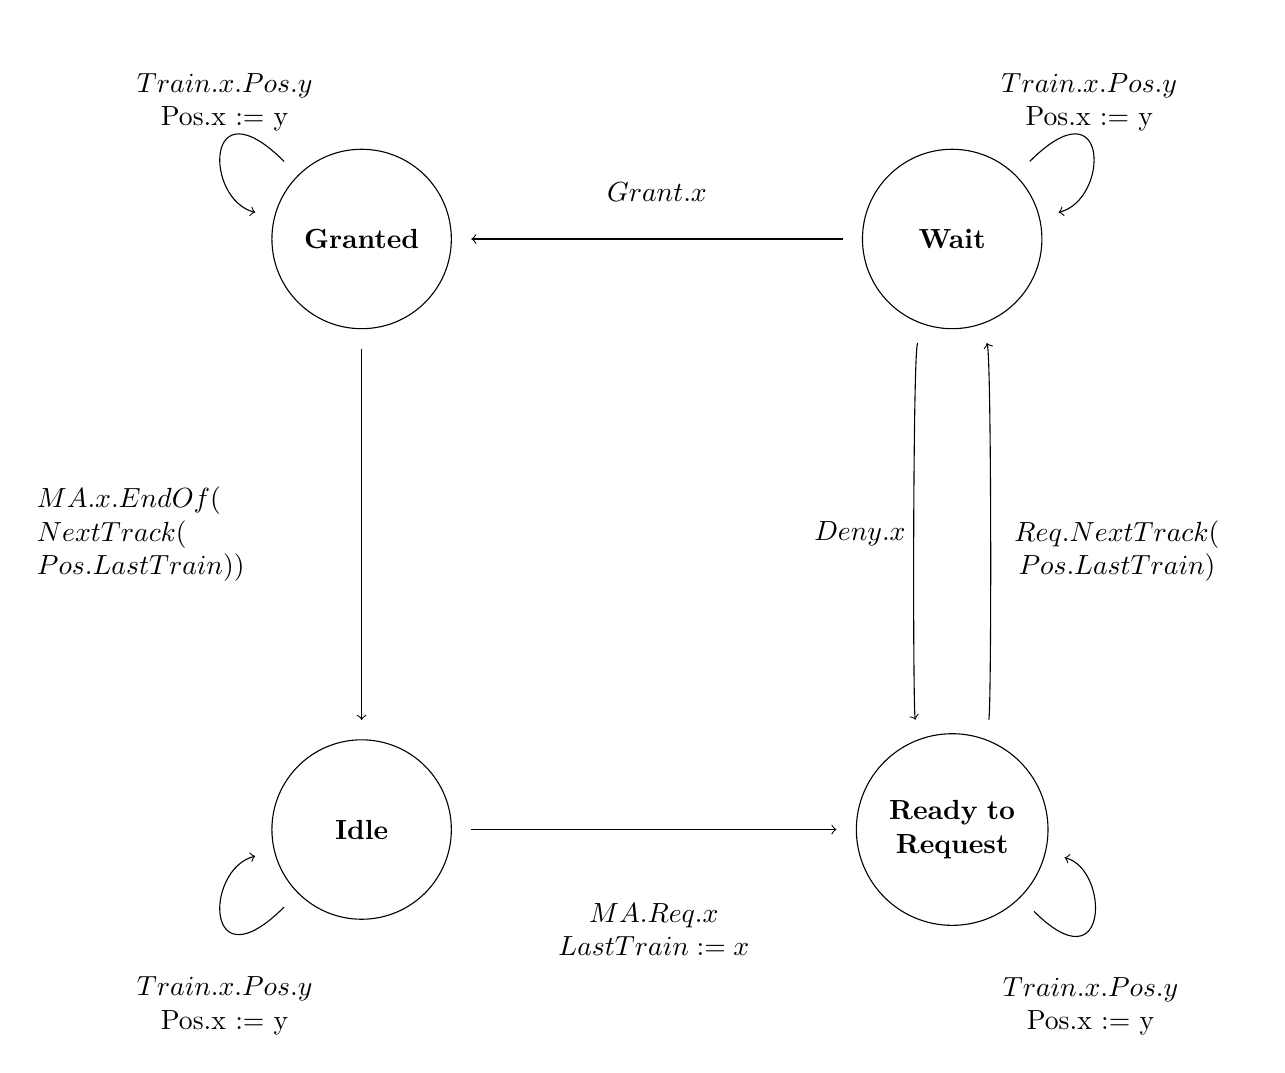
\begin{tikzpicture}[node distance = 1cm]
\tikzstyle{box1}=[circle, draw, text width = 2cm, text centered ]
\tikzstyle{arrow}=[->,shorten >=7pt,shorten <= 7pt]
\tikzstyle{biarrow}=[<->,very thick,shorten >=7pt,shorten <=7pt]
\node (A) [box1]  at (0,0)                  {\textbf{Idle} };
\node (B) [box1]    at (7.5,0)          {\textbf{Ready to Request} };
\node (C)[box1] at (0, 7.5)  {  \textbf{Granted}  };
\node (D)[box1] at (7.5, 7.5)  { \textbf{Wait} };


\draw [arrow] (B)  .. controls +(0.5cm,  1.5 cm) and +(0.5cm,  -1.5 cm ) .. node[right, text width = 3cm] {\begin{center}$Req.NextTrack($ \\ $Pos.LastTrain)$ \end{center}} (D);
\draw [arrow] (D) .. controls +(-0.5cm,  -1.5cm) and +(-0.5cm, 1.5 cm ) ..   node [left] {$Deny.x$} (B);
\draw [arrow] (A) -- node[below = 10pt, text width = 4cm] {\begin{center}$MA.Req.x$ \\ $LastTrain := x$\end{center}} (B);
\draw [arrow] (D) --  node[above = 10pt,text width=4cm] {\begin{center}$Grant.x$\end{center}} (C);
\draw [arrow] (C) -- node [left, text width = 4cm] {$MA.x.EndOf($ \\ $NextTrack($ \\ $Pos.LastTrain))$} (A);

\draw [arrow] (C) .. controls +(-2cm,  2cm) and +(-2cm, 0.5 cm ) ..   node [above = 5pt, text width = 4cm] {\begin{center}$Train.x.Pos.y$\\ Pos.x := y\end{center}} (C);
\draw [arrow] (D) .. controls +(2cm,  2cm) and +(2cm, 0.5 cm ) ..   node [above = 5pt, text width = 4cm] {\begin{center}$Train.x.Pos.y$\\ Pos.x := y\end{center}} (D);
\draw [arrow] (B) .. controls +(2cm,  -2cm) and +(2cm, -0.5 cm ) ..   node [below = 6pt, text width = 4cm] {\begin{center}$Train.x.Pos.y$\\ Pos.x := y\end{center}} (B);
\draw [arrow] (A) .. controls +(-2cm,  -2cm) and +(-2cm, -0.5 cm ) ..   node [below = 6pt, text width = 4cm] {\begin{center}$Train.x.Pos.y$\\ Pos.x := y\end{center}} (A);


\end{tikzpicture} 
\end{center}
\caption{Radio Block Processor Automaton}
\label{fig:RBCAuton}
\end{figure}

\end{document}
